% !TEX root = ../Thesis.tex
\chapter{Related Work}
\label{ch:related-work}

\begingroup
\setaftersecskip{6pt}
\setlength{\emergencystretch}{2em}
This chapter explains how the thesis relates to previous research on virtual exhibitions and immersive search systems. It considers three areas that are important for the developed VR museum: virtual exhibitions, immersive multimedia retrieval and content-based exploration of virtual museums. Previous works cover individual parts of these areas. However, none of the reviewed works combines cross-media search, the dynamic creation of an exhibition and its continued exploration in an interactive VR museum.

\section{Virtual Exhibitions}
\label{sec:related-virtual-exhibitions}

Virtual exhibitions solve a space problem. Digital collections can be much larger than the physical exhibition space that is available. In a virtual environment, the same objects can be used in different groups and can be accessed independently of their physical location. Two systems developed at the University of Basel are especially relevant to this thesis.

\paragraph{VIRTUE}
VIRTUE is a system for creating and viewing virtual exhibitions. An administrative interface allows users to create rooms and place images, videos and 3D artifacts. The exhibition is built with Unity and can then be visited in the VR frontend. Exhibitions, artifacts and their metadata are stored centrally in MongoDB. The system therefore follows a clear process. First, an exhibition is created manually. It is then viewed in VR. VIRTUE shows that a multimodal VR museum is technically possible, but it does not create an exhibition from a search query \citep{giangreco2019virtue}.

\paragraph{Automatic Gallery Generation}
\citet{peterhans2022galleries} extend VIRTUE with the automatic creation of image galleries. The extended architecture consists of the Virtual Reality Exhibition Presenter (VREP), the web-based Virtual Reality Exhibition Manager User Interface (VREM-UI) and the Virtual Reality Exhibition Manager (VREM). VREM manages the exhibitions in MongoDB and provides them to the VR frontend through a REST interface. To create the galleries, VREM is connected to Cineast. The extracted image features are then stored in Cottontail DB. The components and their interfaces are shown in Figure~\ref{fig:virtue-architecture} \citep{peterhans2022galleries}.

\begin{figure}[htbp]
  \centering
  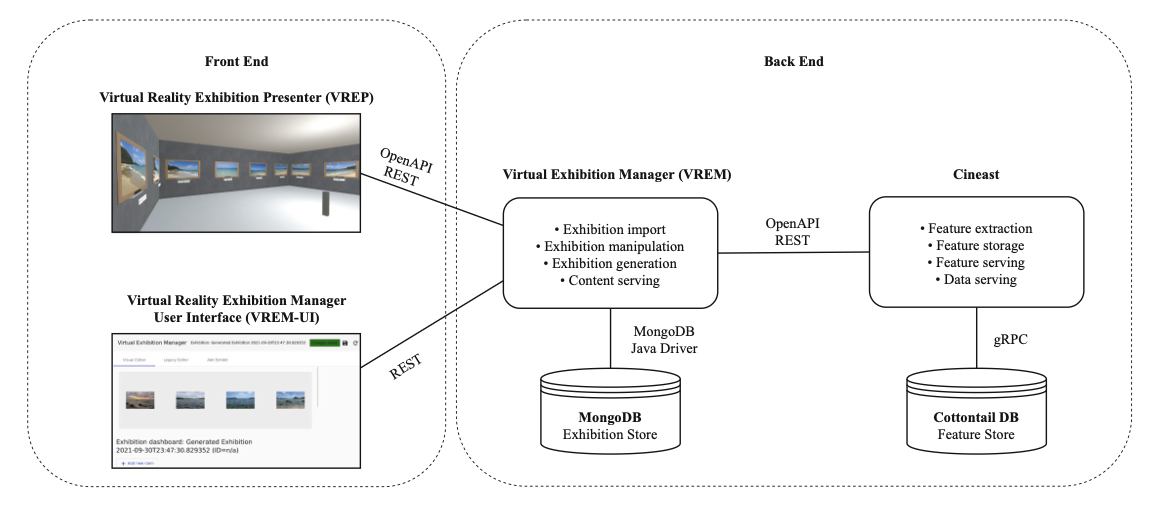
\includegraphics[width=\textwidth]{Figures/ch02-01-virtue-architecture.png}
  \caption[Architecture of VIRTUE with automatic gallery generation]{
    Architecture of VIRTUE with the extension for automatic image gallery creation \protect\citep[Fig.~1]{peterhans2022galleries}.
  }
  \label{fig:virtue-architecture}
\end{figure}

For the arrangement, the system trains a Self-Organizing Map on image features extracted earlier. Each node is assigned a representative image. When this image is selected, a sub-room with more images assigned to the same node is created \citep{peterhans2022galleries}.

\paragraph{Space-Adaptive Artwork Placement}
\citet{kim2024spaceadaptive} follow an approach that focuses more on curating the exhibition. The system creates thematic groups of artworks and uses five adjustable content-similarity factors: color, material, description, artist and production date. An algorithm then determines the placement using four cost functions: intra-cluster distance, inter-cluster distance, intra-cluster intervisibility and occupancy. The process is summarized in Figure~\ref{fig:space-adaptive-placement}.

\begin{figure}[htbp]
  \centering
  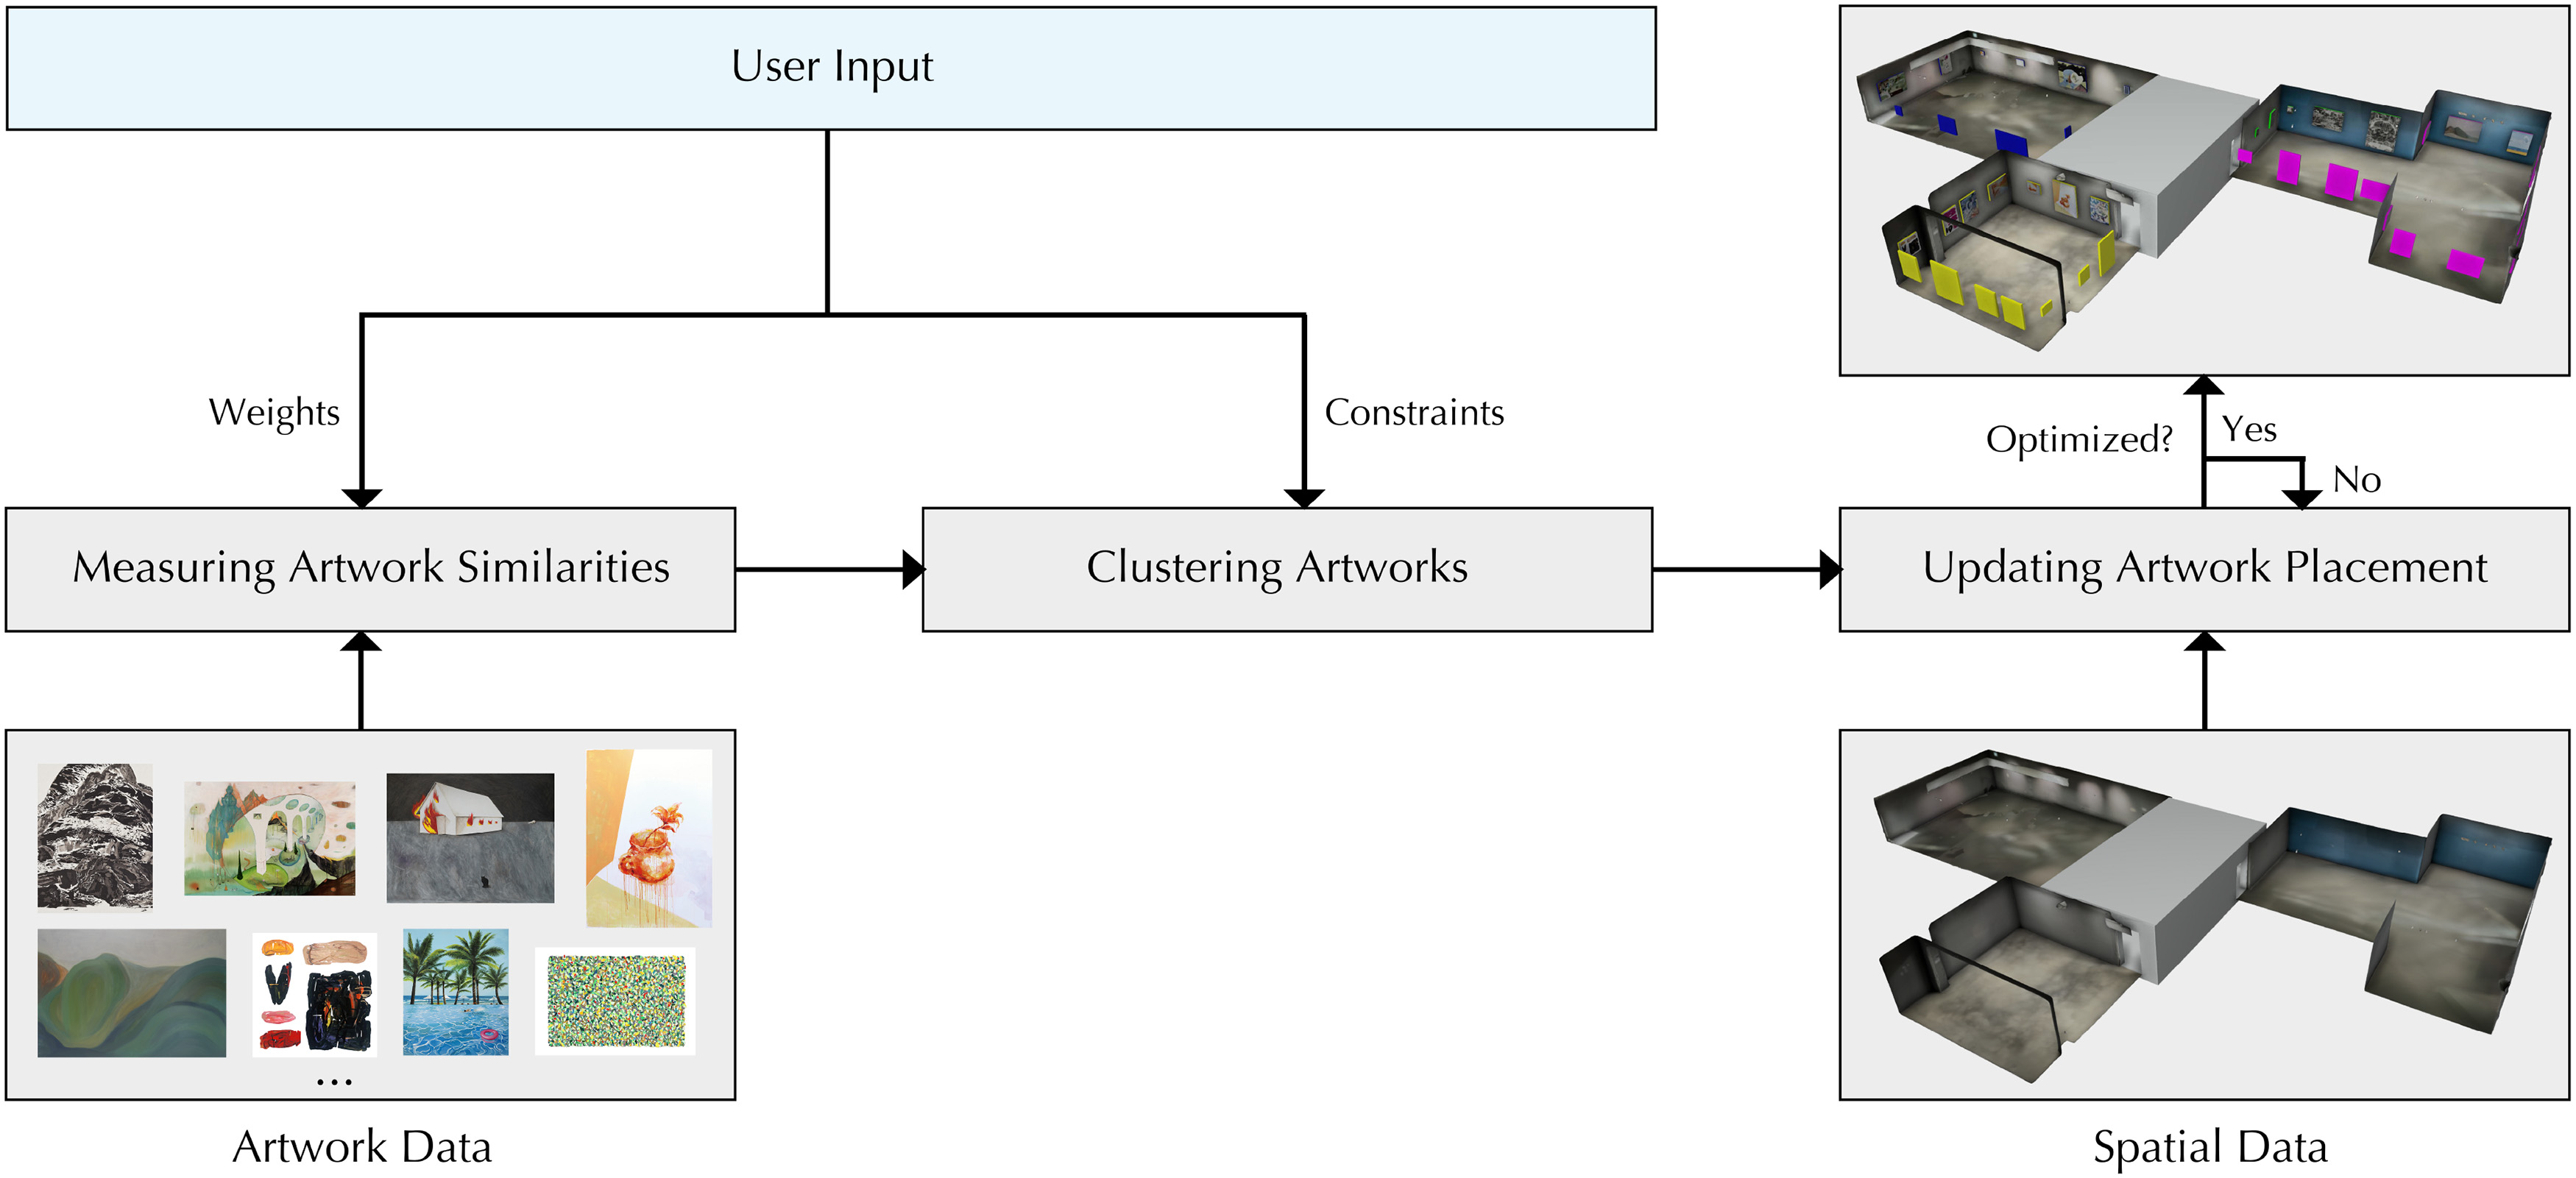
\includegraphics[width=\textwidth]{Figures/ch02-02-space-adaptive-placement.png}
  \caption[Workflow of space-adaptive artwork placement]{
    Similarity-based grouping followed by improved placement based on spatial rules \protect\citep[Fig.~1]{kim2024spaceadaptive}.
  }
  \label{fig:space-adaptive-placement}
\end{figure}

\clearpage
These works create exhibitions that are ordered by content or improved for the available space. The prototype developed here follows a different approach. Instead of curating an exhibition in advance, it builds a temporary exhibition from an already ranked result set from the vitrivr-engine. A new text or similarity query replaces this exhibition and continues the exploration at a new point in the collection.

\section{Immersive Multimedia Retrieval}
\label{sec:related-immersive-retrieval}

The second research area uses immersive environments mainly as user interfaces for multimedia retrieval, not as exhibition spaces. Both the creation of a query and the presentation and study of its results are moved into three-dimensional space.

\paragraph{vitrivr-VR}
vitrivr-VR is a fully immersive user interface for video search. The version described in 2022 uses Cottontail DB for storage and similarity search, Cineast for feature extraction and query processing and a VR frontend developed in Unity. The components communicate through the Cineast REST interface \citep{spiess2022vitrivrvr}.

The system supports several types of queries: concept, text, Boolean, geographic, temporal and pose queries. Users enter text through an offline speech-to-text tool. The results appear on a cylindrical surface \citep{spiess2022vitrivrvr}. vitrivr-VR therefore shows how immersive forms of querying and result analysis can extend an existing retrieval system. This thesis follows the same basic idea. However, it only supports text and similarity queries, and it presents the results as an exhibition that users can walk through.

\paragraph{MediaMix}
MediaMix moves multimedia retrieval from a fully virtual environment into an MR environment\footnote{\emph{Mixed Reality} (MR) combines the visible real environment with spatially embedded digital content that users can interact with.}. The application uses the Apple Vision Pro and places search interfaces and results in the physical space. Its backend is the modular vitrivr-engine, which is connected to PostgreSQL and pgvector in the 2025 version. Figure~\ref{fig:mediamix-architecture} shows the separation into frontend, retrieval engine and database \citep{arnold2025mediamix}.

\clearpage
\begin{figure}[htbp]
  \centering
  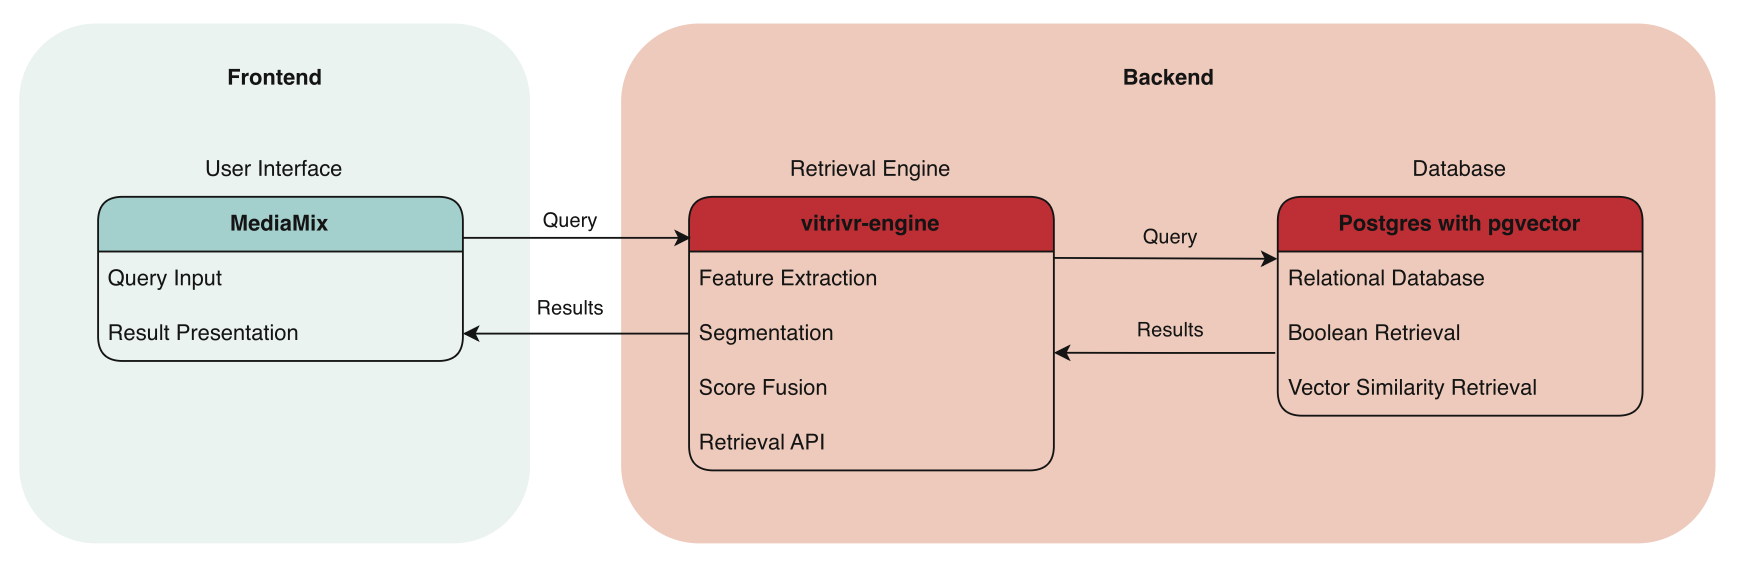
\includegraphics[width=\textwidth]{Figures/ch02-03-mediamix-architecture.png}
  \caption[Architecture overview of the MediaMix stack]{
    Architecture overview of the MediaMix stack \protect\citep[Fig.~1]{arnold2025mediamix}.
  }
  \label{fig:mediamix-architecture}
\end{figure}

Text queries can be entered with a physical keyboard or Apple's speech-to-text service. Similarity queries use individual video frames and CLIP or DINO features\footnote{DINO stands for \emph{self-distillation with no labels} and is a self-supervised method for creating visual features.}. CLIP is explained in Section~\ref{sec:background-clip}. Each query creates its own result sphere, which stays in the room. This allows earlier and current searches to be studied side by side \citep{arnold2025mediamix}. MediaMix and this thesis therefore both use a vitrivr backend and spatial retrieval interfaces. In the VR museum, images, videos and 3D models are presented together as exhibits and explored through a series of queries.

\section{Content-Based Exploration in Virtual Museums}
\label{sec:related-content-exploration}

Systems in which a search query, a selected exhibit or observed behavior starts further exploration are especially close to the idea of this thesis.

\paragraph{Query-Based Exhibition Generation}
\citet{hayashi2020internet} already implement a direct process from a search query to a virtual exhibition. The application accepts keywords for fields in the Metropolitan Museum of Art's Open Access database, downloads the matching artwork images and automatically shows them in a 3D museum that visitors can move through freely. The basic idea of a search-based exhibition therefore already exists. However, this short system paper is limited to artwork images and metadata from a single external collection. It does not cover cross-media search or further exploration through an exhibited result.

\paragraph{Content-Based Navigation}
\citet{koutsoudis2012navigation} connect a web-based virtual museum with a content-based search for 3D artifacts. The project contains 61 vessel models: six were digitized, while the remaining 55 were modeled by hand. Visitors can rotate an exhibited vessel, view information about it and use it for a query by example. A server then calculates the similarity of its shape to those of the other models. However, the system is a non-immersive application in a web browser, and its search is limited to a uniform collection of 3D vessels.

\paragraph{Virtual Art Exhibition System}
The Virtual Art Exhibition System creates the next exhibition from a person's observed behavior. First, eight artworks are shown in a room. Invisible areas with a radius of two meters measure how long the person stays in front of each image. When the person leaves the room through an exit, the system identifies the work that was viewed for the longest time. It then searches for works related by period, artist and country and uses them to create a new exhibition. This change is shown in Figure~\ref{fig:virtual-art-interest} \citep{fukuda2023virtualart}.

\begin{figure}[htbp]
  \centering
  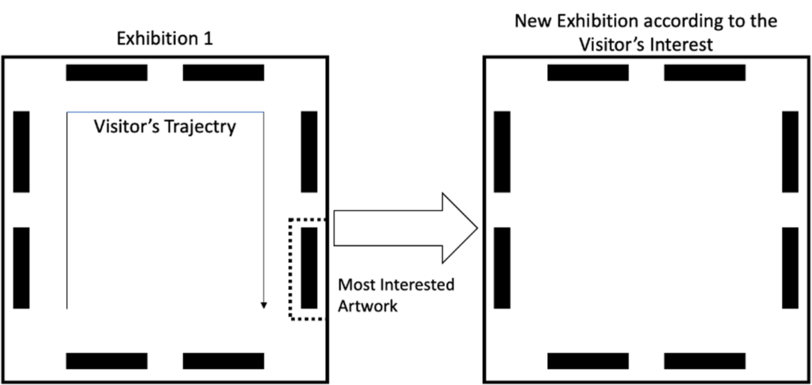
\includegraphics[width=0.82\textwidth]{Figures/ch02-04-virtual-art-interest.png}
  \caption[Generation of an exhibition from visitor interest]{
    Creation of a new exhibition based on the artwork viewed for the longest time \protect\citep[Fig.~2]{fukuda2023virtualart}.
  }
  \label{fig:virtual-art-interest}
\end{figure}

\citet{meinecke2022contextualizing} also focus on continued exploration. Their virtual museum links exhibited works to related images. Filters for artist, style and recognized object classes, as well as several interactive visualizations, offer different ways to access the collection. The work therefore combines a virtual museum, similarity calculation and exploratory search, but it remains an image-based online application.

These works are closer to the interaction model of the VR museum than a general method for 3D model search. They use a text query, a selected exhibit, observed interest or content filters to provide access to more works. This thesis lies where these approaches meet. Like VIRTUE, it presents different media types in VR. Like vitrivr-VR and MediaMix, it uses the retrieval backend. Like the systems for content-based navigation, it allows continued exploration. Its own contribution is to combine these features in one process. An exhibit directly starts a cross-media similarity search, and every result set appears as a new, fully immersive exhibition.

\endgroup
